\section{QCM (3 points)}

Pour chaque question, choisir la (ou les) bonnes réponses

\begin{questions}
	
	\begin{multicols}{2}
		
		\question[\half] Le ballon de handball est en mouvement par rapport :
	
	
	
		
	\begin{checkboxes}
		\correctchoice au sol.
		\correctchoice à un joueur.
		\choice au ballon.
	\end{checkboxes}

	\begin{center}
		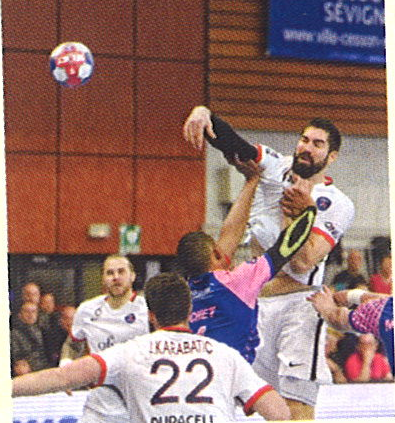
\includegraphics[scale=0.3]{hand}
	\end{center}
	\end{multicols}

	\question[\half] La tour Eiffel est fixe par rapport :\\
	\begin{oneparcheckboxes}
		\choice à la Lune.
		\correctchoice à la surface de la Terre.
		\choice au Soleil
	\end{oneparcheckboxes}

	\question[\half] Les passagers d'une grande roue pendant son fonctionnement sont immobiles par rapport :
	\begin{oneparcheckboxes}
		\correctchoice à leur nacelle.
		\choice au sol.
		\choice au centre de la roue.
	\end{oneparcheckboxes}



	\begin{multicols}{2}
		\question[\half] L'image ci-dessous est une chronophotographie d'un saut en bmx. La trajectoire du casque par rapport au sol est :
	\begin{checkboxes}
		\correctchoice curviligne.
		\choice rectiligne.
		\choice circulaire.
	\end{checkboxes}

	
	\begin{center}
		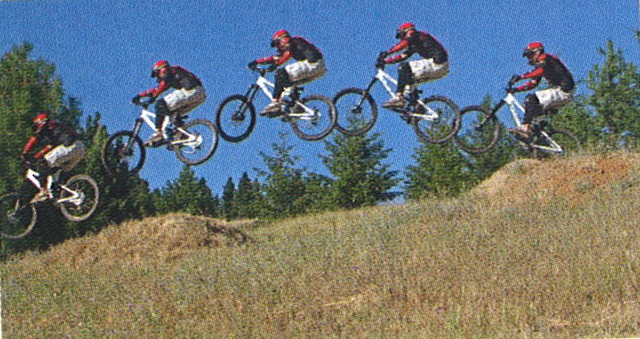
\includegraphics[scale=0.3]{bmx}
	\end{center}

	\end{multicols}
	\question[\half] La trajectoire de la nacelle d'une grande roue par rapport au sol est :\\
	\begin{oneparcheckboxes}
		\choice curviligne.
		\choice rectiligne.
		\correctchoice circulaire.
	\end{oneparcheckboxes}
	
	
	\begin{multicols}{2}
		\question[\half] La trajectoire du casque par rapport au centre de la Terre de ces enfants assis sur un banc est :
	\begin{checkboxes}
		\choice curviligne.
		\choice rectiligne.
		\correctchoice circulaire.
	\end{checkboxes}

	\begin{center}
		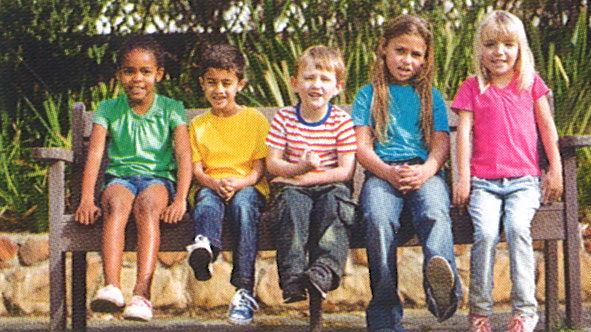
\includegraphics[scale=0.3]{banc}
	\end{center}
	\end{multicols}
\end{questions}